\documentclass[t]{beamer}

% packages
\usepackage[english]{babel}
\usepackage[utf8x]{inputenc}
\usepackage{mathtools}
\usepackage{amsfonts}
\usepackage{amsthm}
\usepackage{numprint}
\usepackage{amsxtra}
\usepackage{amsfonts}
\usepackage{graphicx}
\usepackage{enumerate}
\usepackage{setspace}
\usepackage{booktabs}
\usepackage{tabularx}
\usepackage{amssymb, amstext, amsmath}
\usepackage{fancyhdr}

% macros
% misc
\newcommand\todo[1]{\textcolor{red}{TODO: #1}}
\newcommand\hide[1]{\textcolor{white}{#1}}

% formatting
\newcommand\bld[1]{\textbf{#1}}
\newcommand\ul[1]{\underline{#1}}
\newcommand\n[1]{\numprint{#1}}
\newcommand{\ts}{\textsuperscript}
\newcommand\red[1]{\textcolor{red}{#1}}
\newcommand\blue[1]{\textcolor{blue}{#1}}
\newcommand\link[2]{\href{#1}{\textcolor{blue}{\underline{#2}}}}

% sets
\newcommand\set[1]{\mathcal{#1}}
\newcommand\bb[1]{\mathbb{#1}}
\renewcommand\:{\colon} % for use with \sset, etc.
\newcommand{\sset}[1]{\left\{\,#1\,\right\}} % { ? }, automatic brackets
\newcommand{\ssets}[1]{\left\{#1\right\}} % {?}, automatic brackets
\newcommand{\ssetn}[1]{\{\,#1\,\}} % { ? }, normal brackets

% table formatting
% To better align bold entries in S columns (still broken)
% \usepackage{siunitx}
% \robustify\bfseries
% \newrobustcmd{\bfcell}{\bfseries}

% vector variables (taken from macros by Rainer Gemulla)
\newcommand\vect[1]{{\boldsymbol{#1}}}
\newcommand\va{\vect{a}}
\newcommand\vb{\vect{b}}
\newcommand\vc{\vect{c}}
\newcommand\vd{\vect{d}}
\newcommand\ve{\vect{e}}
\newcommand\vf{\vect{f}}
\newcommand\vg{\vect{g}}
\newcommand\vh{\vect{h}}
\newcommand\vi{\vect{i}}
\newcommand\vj{\vect{j}}
\newcommand\vk{\vect{k}}
\newcommand\vl{\vect{l}}
\newcommand\vm{\vect{m}}
\newcommand\vn{\vect{n}}
\newcommand\vo{\vect{o}}
\newcommand\vp{\vect{p}}
\newcommand\vq{\vect{q}}
\newcommand\vr{\vect{r}}
\newcommand\vs{\vect{s}}
\newcommand\vt{\vect{t}}
\newcommand\vu{\vect{u}}
\newcommand\vv{\vect{v}}
\newcommand\vw{\vect{w}}
\newcommand\vx{\vect{x}}
\newcommand\vy{\vect{y}}
\newcommand\vz{\vect{z}}
\newcommand\vzero{\vect{0}}
\newcommand\vone{\vect{1}}

\newcommand\valpha{\vect{\alpha}}
\newcommand\vbeta{\vect{\beta}}
\newcommand\veps{\vect{\epsilon}}
\newcommand\vdelta{\vect{\delta}}
\newcommand\vtheta{\vect{\theta}}
\newcommand\vsigma{\vect{\sigma}}
\newcommand\vpi{\vect{\pi}}
\newcommand\vlambda{\vect{\lambda}}

% matrix variables (taken from macros by Rainer Gemulla)
\newcommand\mA{\vect{A}}
\newcommand\mB{\vect{B}}
\newcommand\mC{\vect{C}}
\newcommand\mD{\vect{D}}
\newcommand\mE{\vect{E}}
\newcommand\mF{\vect{F}}
\newcommand\mG{\vect{G}}
\newcommand\mH{\vect{H}}
\newcommand\mI{\vect{I}}
\newcommand\mJ{\vect{J}}
\newcommand\mK{\vect{K}}
\newcommand\mL{\vect{L}}
\newcommand\mM{\vect{M}}
\newcommand\mN{\vect{N}}
\newcommand\mO{\vect{O}}
\newcommand\mP{\vect{P}}
\newcommand\mQ{\vect{Q}}
\newcommand\mR{\vect{R}}
\newcommand\mS{\vect{S}}
\newcommand\mT{\vect{T}}
\newcommand\mU{\vect{U}}
\newcommand\mV{\vect{V}}
\newcommand\mW{\vect{W}}
\newcommand\mX{\vect{X}}
\newcommand\mY{\vect{Y}}
\newcommand\mZ{\vect{Z}}
\newcommand\mzero{\vect{0}}

\newcommand{\mPi}{{\ensuremath{\vect{\Pi}}}}
\newcommand{\mSigma}{{\ensuremath{\vect{\Sigma}}}}
\newcommand{\mLambda}{{\ensuremath{\vect{\Lambda}}}}

% argmin, argmax
\DeclareMathOperator*{\argmin}{argmin} % amsmath package required
\DeclareMathOperator*{\argmax}{argmax} % amsmath package required

% matrix operations
\newcommand\xdiag{\operatorname{diag}}      
\newcommand\diag[1]{\xdiag\left(#1\right)}    % diagonal matrix


% new commands
\newcommand\op[1]{\operatorname{#1}}

% choose how your presentation looks.
% for more themes, color themes and font themes, see:
% http://deic.uab.es/~iblanes/beamer_gallery/index_by_theme.html

\mode<presentation>
{%
	\usetheme{default}      % or try Darmstadt, Madrid, Warsaw, ...
	\usecolortheme{default} % or try albatross, beaver, crane, ...
	\usefonttheme{default}  % or try serif, structurebold, ...
	\setbeamertemplate{navigation symbols}{}
	\setbeamertemplate{caption}[numbered]
	% For a numbered table of contents
	\setbeamertemplate{section in toc}[sections numbered] 
	% For slide numbers
	\addtobeamertemplate{navigation symbols}{}{%
	\usebeamerfont{footline}
	\usebeamercolor[fg]{footline}
	\hspace{1em}
	\insertframenumber%/\inserttotalframenumber
	}
} 

%% so table of content appears before each section, highlighting what's next
%\AtBeginSection[]
%{%
%	\setbeamercolor{section in toc shaded}{fg=structure}
%	\begin{frame}<beamer>
%	  \frametitle{Outline}
%	  \tableofcontents[currentsection]
%	\end{frame}
%}

% adds title slides for each section
\AtBeginSection[]{
  \begin{frame}
  \vfill
  \centering
  \begin{beamercolorbox}[sep=8pt,center,shadow=true,rounded=true]{title}
    \usebeamerfont{title}\Huge\insertsectionhead\par%
  \end{beamercolorbox}
  \vfill
  \end{frame}
}

\title[Write your short title here]{Advanced Methods in Text Analytics}
\subtitle{Exercise 7: Large Language Models - Part 1}
\author{Daniel Ruffinelli}
\institute{University of Mannheim}
\date{FSS 2025}

\begin{document}

% no "Figure X" prefix in image captions when using the figure environment
\setbeamertemplate{caption}{\raggedright\insertcaption\par}

\begin{frame}
    \titlepage{}
\end{frame}

\begin{frame}{Transfer Learning}{Question a)}
    \begin{itemize}
        \item What do we mean when we say that a model is ``pre-trained''?
        \item Why don't we say the model is simply ``trained''?
        \item What type of data do we need for pre-training a language model?
    \end{itemize}
\end{frame}

\begin{frame}{Transfer Learning}{Answer a)}
    \begin{itemize}
        \item A model is said to be \emph{pre-trained} when the goal of the
              training process is to learn \emph{general} representations of the
              input data, without a specific downstream task in mind.
        \item In that sense, the prefix ``pre'' indicates that the
              model is trained \emph{before} being fine-tuned on a specific
              task.
        \item In the context of LLMs, fine-tuning is not done as frequently as
              in the era of pre-trained language models (PLMs), e.g.\ BERT.
        \item So we can speak of pre-training as the training of a model before
              it is actually used on a different set of (downstream) tasks.
    \end{itemize}
\end{frame}

\begin{frame}{Transfer Learning}{Question b)}
    \begin{itemize}
        \item What are the two more common training objectives for pre-training
              large language models?
    \end{itemize}
\end{frame}

\begin{frame}{Transfer Learning}{Answer b)}
    \begin{itemize}
        \item Pre-training usually involves training a model on a corpus of data
              using a \emph{self-supervised} learning objective.
        \item Most common ones are: (i) causal language modeling (CLM) and (ii)
              masked language modeling (MLM).
    \end{itemize}
\end{frame}

\begin{frame}{Transfer Learning}{Question c)}
    \begin{itemize}
        \item Let $S$ be the set of sequences used for training language model
              $p$.
        \item Using $p$ and $S$, give formal definitions for the training
              objectives mentioned in your previous answer.
    \end{itemize}
\end{frame}

\begin{frame}{Transfer Learning}{Answer c) (1)}
    \begin{itemize}
        \item The CLM objective is defined as follows:
              \begin{align}
                  \op{CLM}(S) & = \prod_{s=1}^{S} p(x_{|s|} \mid x_1, x_2, \ldots, x_{|s|-1}),
              \end{align}
              where $x_i$ are tokens in sequence $s$.
        \item Similarly, the MLM objective is defined as follows:
              \begin{align}
                  \op{MLM}(S) & = \prod_{s=1}^{S} \prod_{m=1}^{M_s} p(x_m \mid x_1, x_2, \ldots, x_{|s|} \setminus M),
              \end{align}
              where $M_s$ is set of masked out tokens in sequence $s$ and
              $A \setminus B$ is set difference.
    \end{itemize}
\end{frame}

\begin{frame}{Transfer Learning}{Answer c) (2)}
    \begin{itemize}
        \item In practice, we use empirical risk minimization with log loss during
              training.
        \item That is,
              \begin{align}
                  \op{CLM}(S) & = - \frac{1}{|S|} \sum_{s=1}^{S} \log p(x_{|s|} \mid x_1, x_2, \ldots, x_{|s|-1}),
              \end{align}
              \begin{align}
                  \op{MLM}(S) & = - \frac{1}{|M|} \sum_{s=1}^{S} \sum_{m=1}^{M_s} \log p(x_m \mid x_1, x_2, \ldots, x_{|s|} \setminus M),
              \end{align}
              where $M = \{M_1 \cup M_2 \cup \ldots \cup M_{|S|}\}$ is set of
              all masked tokens in $S$.
    \end{itemize}
\end{frame}

\begin{frame}{Transfer Learning}{Question d)}
    \begin{itemize}
        \item What type of data should we use for pre-training an LLM?
        \item What factors should we consider when choosing what data to train
              on?
    \end{itemize}
\end{frame}

\begin{frame}{Transfer Learning}{Answer d)}
    \begin{itemize}
        \item The main factors are: (i) size, (ii) quality, and (iii) domain.
        \item \textbf{Size.} The data should be large enough to capture wide
              range of linguistic patterns/concepts, allowing model to
              learn rich set of representations.
        \item It should also be large enough to avoid overfitting, easily done
              with a large number of parameters.

        \item \textbf{Quality}. Also important, but it can be
              measured in different ways.
              E.g.\ grammatical correctness, lexical variety, etc.
              What is good quality usually depends on goal with model.
        \item E.g.\ if goal is to train a model for speaking formal English,
              then University textbooks are likely a high quality source.
        \item But if goal in on colloquial English, then online forums are
              likely a better source.

        \item \textbf{Domain.} Pre-training data should be a diverse collection
              of text from various sources that cover a set of domains of
              interest, e.g.\ medicine, biology, pop culture, etc.
    \end{itemize}
\end{frame}

\begin{frame}{Transfer Learning}{Question e)}
    \begin{itemize}
        \item We typically talk of fine-tuning a pre-trained model.
        \item What do we mean by fine-tuning?
        \item How is it different from ``pre-training'' a model?
        \item What type of data do we need for fine-tuning a language model?
    \end{itemize}
\end{frame}

\begin{frame}{Transfer Learning}{Answer e)}
    \begin{itemize}
        \item Fine-tuning refers to process of adapting a pre-trained model to a
              specific downstream task by updating its parameters
              on a smaller labeled dataset that represents this task.
        \item Thus, fine-tuning is different from pre-training in that
              pre-training involves training a model without a specific
              \emph{target} task in mind.

        \item Fine-tuning typically relies on supervised data that represents
              downtream task of interest, e.g.\ pairs of the form
              (review, sentiment) for sentiment analysis of product reviews.
        \item Thus, during fine-tuning, the model should learn task-specific
              patterns and improve its performance on the downstream task, at
              the potential cost of catastrophically forgetting what was learned
              during pre-training.
    \end{itemize}
\end{frame}

\begin{frame}{Transfer Learning}{Question f)}
    \begin{itemize}
        \item What is the main challenge behind traning models with a large
              number of parameters?
    \end{itemize}
\end{frame}

\begin{frame}{Transfer Learning}{Answer f)}
    \begin{itemize}
        \item The main challenge behind training models with a large number of
              parameters is the computational cost and memory requirements that
              come with the training process.
        \item To reduce runtime costs, specialized hardware is commonly used for
              training models, e.g.\ GPUs that are more efficient at computing
              common operations used during training, such as matrix products.
        \item In addition, large models can be memory-intensive, requiring large
              amounts of memory just to store the model parameters and
              intermediate activations during training (as computed soon in
              Task 3).
    \end{itemize}
\end{frame}

\begin{frame}{Parameter Efficient Fine-Tuning}{Context}
    \begin{itemize}
        \item Given the large number of parameters in LLMs, a set of methods
              have focused on fine-tuning large-size models by tuning only a
              subset of their parameters.
        \item In this task, we go over some of the concepts behind such
              parameter efficient fine-tuning (PEFT) methods.
    \end{itemize}
\end{frame}

\begin{frame}{Parameter Efficient Fine-Tuning}{Question a)}
    \begin{itemize}
        \item What is the main idea behind parameter-efficient fine-tuning
              (PEFT)?
        \item Briefly describe two different PEFT methods.
    \end{itemize}
\end{frame}

\begin{frame}{Parameter Efficient Fine-Tuning}{Answer a) (1)}
    \begin{itemize}
        \item Parameter-efficient fine-tuning (PEFT) method aim to reduce the
              computational cost and memory requirements of fine-tuning large
              language models by updating only a subset of the parameters in the
              pre-trained model.
        \item One common approch is the use of \bld{adapters}, which are small
              parameterized components added to the pre-trained architecture,
              typically a transformer-based LM, which modify the model's forward
              pass.
        \item Then, during fine-tuning, only the parameters of the adapters are
              updated, while the parameters of the pre-trained model are kept
              \emph{frozen}.
        \item Adapters can be placed anywhere in the model's architecture and
              thus have different impacts on the forward pass.
        \item In addition, adapters can themselves be somewhat involved, e.g.\
              by including an attention mechanism.
    \end{itemize}
\end{frame}

\begin{frame}{Parameter Efficient Fine-Tuning}{Answer a) (2)}
    \begin{itemize}
        \item Another approach to PEFT is \bld{prompt tuning}, which adds a
              small number of task-specific tokens to the input sequence during
              fine-tuning.
        \item These tokens are used to guide the model towards the task of
              interest, e.g.\ by specifying the task in the promp given to the
              model, e.g. ``summarize this:''
        \item During fine-tuning, only these special tokens are updated, giving
              the model a small set of parameters that can be used to modify its
              outputs to better fit the downstream task of interest.
    \end{itemize}
\end{frame}

\begin{frame}{Parameter Efficient Fine-Tuning}{Question b)}
    \begin{itemize}
        \item Let $\mX = \{\vx_1,\ldots,\vx_n\}$ be the input sequence and
              $\mH = \{\vh_1,\ldots, \vh_n\}$ the corresponding output sequence
              of the FNN operator in a transformer block, where $\op{FNN}(\mX)$
              is parameterized by $\mW_{up}\in\bb{R}^{d\times 4d}$ and
              $\mW_{down}\in\bb{R}^{4d\times d}$, i.e.\ the up and down
              projections in FNN, respectively.
        \item In other words, $\mH = \op{FNN}(\mX\mid \mW_{up}, \mW_{down})$
              (note that we omit biases and the residual connection for
              simplicity).
        \item Give a formal expression for the output of this FNN operator.
    \end{itemize}
\end{frame}

\begin{frame}{Parameter Efficient Fine-Tuning}{Answer b)}
    \begin{itemize}
        \item We have:
              \begin{align}
                  \op{FNN}(\mX) & = f(\mX\mW_{up})\mW_{down},
              \end{align}
              where $f$ is a non-linear activation function, originally ReLU,
              lately different ones like SwiGLU.
    \end{itemize}
\end{frame}

\begin{frame}{Parameter Efficient Fine-Tuning}{Question c)}
    \begin{itemize}
        \item Following the previous subtask, assume we fine-tune the FNN
              operator using the Houlsby adapters introduced in the lectures,
              and call this fine-tuned operator FNN'.
        \item Give a formal expression for FNN' given input sequence $\mX$
              (don't use any biases in the adapter).
        \item Make sure to formally define all parameters introduced by the
              adapter as well as their exact sizes.
        \item What are the hyperparameters used in these adapters? How are these
              hyperparameters typically set?
    \end{itemize}
\end{frame}

\begin{frame}{Parameter Efficient Fine-Tuning}{Answer c)}
    \begin{itemize}
        \item Let $\mA \in \bb{R}^{d\times r}$, $\mB \in R^{r\times d}$ be
              projection matrices in adapter.
        \item Then:
              \begin{align}\label{houlsby}
                  \op{FNN'}(\mX) & =  \op{FNN}(\mX) + g(\op{FNN}(\mX)\mA)\mB,
              \end{align}
              where $g$ is a non-linear activation function (multiple ones were
              originally tested).
        \item That is, Houlsby adapters are applied sequentially after the
              operator being fine-tuned, and they include a residual connection
              as with the other components in the transformer block (hence the
              addition).
        \item Thus, Houslby adapters effectively add a new \emph{sequential}
              component to each transformer block.
        \item Each adapter has $2dr$ number of parameters, where $r$ is
              a hyperparameter, the bottleneck dimension used to control the
              size/capacity of the adapter.
        \item Typically, $r << d$ to keep number of trainable parameters
              low.
    \end{itemize}
\end{frame}

\begin{frame}{Parameter Efficient Fine-Tuning}{Question d)}
    \begin{itemize}
        \item Can Houlsby adapters only be applied to FNN operators?
        \item Why or why not?
    \end{itemize}
\end{frame}

\begin{frame}{Parameter Efficient Fine-Tuning}{Answer d)}
    \begin{itemize}
        \item Houlsby adapters can be placed after any layer or sublayer in the
              model.
        \item In fact, Houlsby originally added one adapter after the
              multi-head attention operator and another after the FNN operator
              in each transformer block.
    \end{itemize}
\end{frame}

\begin{frame}{Parameter Efficient Fine-Tuning}{Question e)}
    \begin{itemize}
        \item Now assume we fine-tune \emph{only} the up projection of the FNN
              operator using LoRA adapters.
        \item Give a formal expression for FNN' given input sequence $\mX$
              (again, no biases in the adapter).
        \item Make sure to formally define all parameters introduced by LoRA as
              well as their exact sizes.
        \item As before, specify the hyperparameters used in LoRA adapters and
              say how they are typically set.
    \end{itemize}
\end{frame}

\begin{frame}{Parameter Efficient Fine-Tuning}{Answer e)}
    \begin{itemize}
        \item Let $\mA \in \bb{R}^{d\times r}$, $\mB \in R^{r\times d}$ be the
              projection matrices in the LoRA adapter.
        \item Then:
              \begin{align}\label{lora}
                  \op{FNN'}(\mX) & = (\mX\mW_{up} + \mX\mA\mB)\mW_{down}
              \end{align}
        \item The addition comes from the LoRA adapter, which is applied using a
              residual connection around the weight matrix we are fine-tuning.
        \item Each adapter has $2dr$ number of parameters, where $r << d$ is
              the hyperparameter that controls the rank of both projection
              matrices used by LoRA adapters.
    \end{itemize}
\end{frame}

\begin{frame}{Parameter Efficient Fine-Tuning}{Question f)}
    \begin{itemize}
        \item Can LoRA adapters only be applied to FNN operators?
        \item Why or why not?
    \end{itemize}
\end{frame}

\begin{frame}{Parameter Efficient Fine-Tuning}{Answer f)}
    \begin{itemize}
        \item LoRA adapters can be applied to any projection matrix, e.g.\ the
              projections used in self-attention layers.
        \item This should be clear from the fact that in the FNN operator, we
              applied a LoRA adapter only to one of the two possible projection
              matrices.
        \item In fact, in the original paper, LoRA adapters were applied to
              matrices $\mW^Q$ and $\mW^V$ in self-attention layers.
    \end{itemize}
\end{frame}

\begin{frame}{Parameter Efficient Fine-Tuning}{Question g)}
    \begin{itemize}
        \item If you haven't already, show that the application of LoRA adapters
              can be expressed as follows:
              \begin{align}
                  \op{FNN'}(\mX) & = \mX(\mW_{up} + \Delta\mW_{up})\mW_{down},
              \end{align}
              where $\Delta\mW_{up}$ is the update introduced during
              fine-tuning.
        \item What is the advantage of this formulation?
        \item Can Houlsby adapters be expressed in a similar way?
    \end{itemize}
\end{frame}

\begin{frame}{Parameter Efficient Fine-Tuning}{Answer g) (1)}
    \begin{itemize}
        \item This is easy to see from Eq.~\ref{lora} and the fact
              that matrix products are distributive w.r.t.\ matrix sum.
              That is,
              \begin{align}
                  \op{FNN'}(\mX) & = (\mX\mW_{up} + \mX\mA\mB)\mW_{down} = \mX(\mW_{up} + \mA\mB)\mW_{down}
              \end{align}
              where $\Delta\mW_{up} = \mA\mB$.
        \item Advantage of this formulation: allows to see that
              learned adapters can be added back into original model after
              fine-tuning is done.
        \item This results in fine-tuned model without increase in number of
              parameters and without corresponding additional runtime costs in
              forward pass.
        \item It also allows for modularity: can we choose (i) which weight
              matrices to tune, and (ii) allows us to remove effect
              of the adapters from model by simply subtracting $\mA\mB$ from
              tuned weight matrix to recover original model.
    \end{itemize}
\end{frame}

\begin{frame}{Parameter Efficient Fine-Tuning}{Answer g) (2)}
    \begin{itemize}
        \item Such advantages not immediately possible with Houlsby adapters.
        \item For one, they were designed to behave similarly to sublayers in
              transformer block, so it's not clear what impact they would have
              when applied to, e.g., matrix $\mW^K$ in a self-attention layer.
        \item In addition, Houlsby adapters make changes to residual space using
              linear projections that include a non-linear activation function
              in between.
        \item So if we want to remove impact of these adapters to
              recover original model, we would have to ensure non-linear
              activation function has an inverse function and that the learned
              projections are invertible.
    \end{itemize}
\end{frame}

\begin{frame}{Transformer-Based LLMs}{Context}
    \begin{itemize}
        \item In this task, we discuss the main components of a
              transformer-based large language model (LLM).
        \item In particular, we focus on a causal language model (CLM) similar
              to the GPT-3 model released
              by~\link{https://arxiv.org/pdf/2005.14165}{Brown et al. (2020)}.
    \end{itemize}
\end{frame}

\begin{frame}{Transformer-Based LLMs}{Question a)}
    \begin{itemize}
        \item Why do transformer-based language models require positional
              encodings?
        \item Given a language model with $L$ transformer layers, how many
              positional encoding layers does this model use?
    \end{itemize}
\end{frame}

\begin{frame}{Transformer-Based LLMs}{Answer a) (1)}
    \begin{itemize}
        \item Positional encodings are required to provide the transformer model
              with information about position of each token in the input
              sequence.
        \item This is because the transformer architecture does not have any
              built-in mechanism to understand the order of the tokens in the
              input sequence, unlike RNNs which process tokens sequentially,
              thus naturally having a ``sense of time''.
        \item Positional encodings are \emph{typically} added to input
              embeddings before feeding them into the first transformer layer.
        \item Thus, a language model with $L$ transformer layers uses a single
              positional encoding layer, independently of the number of
              transformer layers in the model.
        \item However, some positional encoding layers are added to each
              transformer layer.
    \end{itemize}
\end{frame}

\begin{frame}{Transformer-Based LLMs}{Answer a) (2)}
    \begin{itemize}
        \item Recall from lecture: LMs as stacked layers of transformers
    \end{itemize}
    \begin{center}
        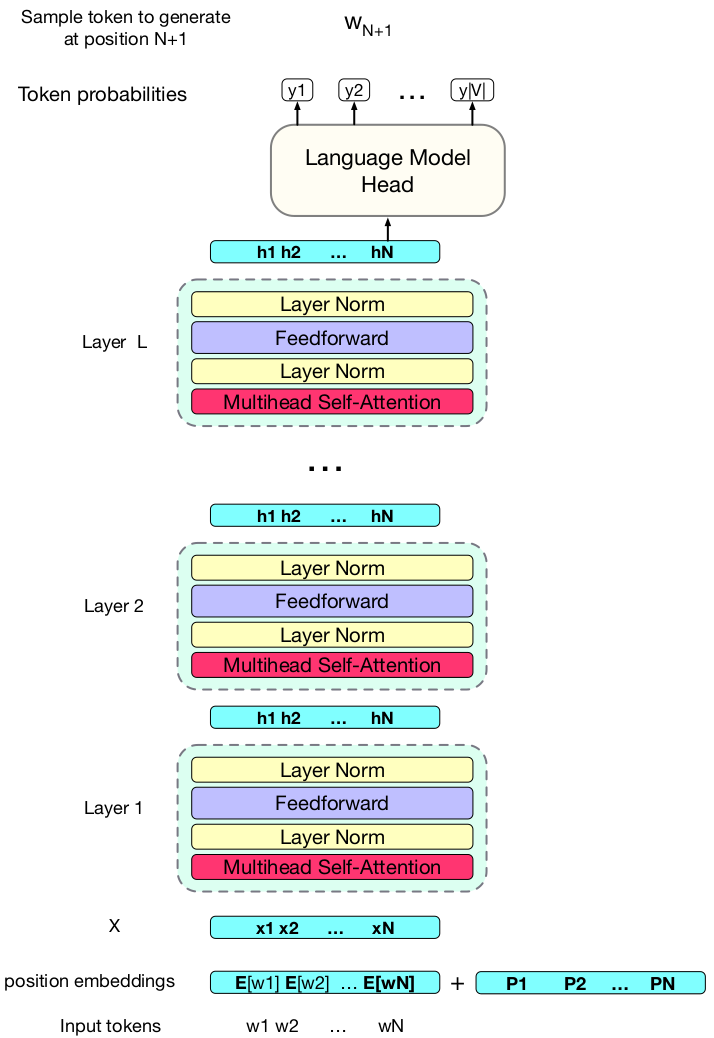
\includegraphics[scale=0.2]{img/stacked_transformers.png}
    \end{center}
\end{frame}

\begin{frame}{Transformer-Based LLMs}{Question b)}
    \begin{itemize}
        \item What is the role of the language model head in a transformer-based
              language model?
        \item What sort of ``weight tying'' is typically used with the language
              model head?
    \end{itemize}
\end{frame}

\begin{frame}{Transformer-Based LLMs}{Answer b)}
    \begin{itemize}
        \item \bld{LM head in an LM:} responsible for producing the distribution
              used for predicting the next token given an input sequence.
        \item \bld{Common implementation:} softmax layer that projects
              contextualized (hidden) representations of the input tokens to
              the vocabulary space and applies softmax function to normalize
              logit scores into a probability distribution.
        \item \bld{Weight tying:} weights of language model head are typically
              tied to (static) input embeddings, because both (static) embedding
              matrix and projection matrix in the LM head are of the same size.
        \item I.e., the weights of the language model head are the
              same as the weights of the input embeddings.
        \item This weight tying helps in reducing the number of parameters in
              the model and improves the generalization of the model.
    \end{itemize}
\end{frame}

\begin{frame}{Transformer-Based LLMs}{Question c)}
    \begin{itemize}
        \item As done in previous exercises, give a formal expression for the
              output of a multi-head attention operator $\op{MHA}$ that uses $n$
              self-attention heads $\op{SA}_i$?
        \item What are the parameters $\vtheta_{\op{MHA}}$ assuming each
              $\op{SA}_i$ operator is parameterized by $\vtheta_{\op{SA}_i}$?
    \end{itemize}
\end{frame}

\begin{frame}{Transformer-Based LLMs}{Answer c)}
    \begin{itemize}
        \item The output of a multi-head attention operator $\op{MHA}$ that uses
              $n$ self-attention heads $\op{SA}_i$ is the concatenation of the
              outputs of each head.
        \item To ensure the size of the output is the same as the input, these
              concatenated outputs are projected to the same size as the input.
        \item That is,
              \begin{align}\label{eq:mha}
                  \op{MHA} = (\op{SA}_1 \oplus \op{SA}_2 \oplus \ldots \oplus \op{SA}_n)\mW^O,
              \end{align}
              where $\oplus$ denotes the concatenation operation.
        \item The parameters of the multi-head attention operator are the
              parameters of each attention head plus the output projection
              matrix $\mW^O$.
        \item In other words,
              \begin{align}
                  \vtheta_{\op{MHA}} = [\vtheta_{\op{SA}_1}, \vtheta_{\op{SA}_2}, \ldots, \vtheta_{\op{SA}_n}, \mW^O].
              \end{align}
    \end{itemize}
\end{frame}

\begin{frame}{Transformer-Based LLMs}{Question d)}
    \begin{itemize}
        \item Assume you have a pre-trained causal language model $\op{CLM}$
              parameterized by $\vtheta_{CLM}$.
        \item The model is implemented with transformers and follows the GPT-3
              architecture, meaning the size of the input and output
              representations in each transformer layer is $d_H = 12288$.
        \item If each attention head projects input representations to dimension
              $d_{\op{SA}_i} = 128$ and the projection \emph{inside} the
              multi-head attention operator $\op{MHA}$ does not change the
              dimension of its inputs, how many attention heads does each
              $\op{MHA}$ operator have?
        \item Give a numeric answer and show the calculations that lead to your
              answer.
        \item \textbf{Hint:} remember that the size of the output
              representations of a $\op{MHA}$ operator are also the same size as
              its input representations.
    \end{itemize}
\end{frame}

\begin{frame}{Transformer-Based LLMs}{Answer d) (1)}
    \begin{itemize}
        \item Let's start with what we know.
              \begin{enumerate}
                  \item The output of each self-attention layer $\op{SA}_i$ is
                        of size $128$.
                  \item The size of the output representations of a $\op{MHA}$
                        operator are the same size as the input representations,
                        in this case $d_H = 12288$.
                  \item The $\op{MHA}$ operation is given by Eq.~\ref{eq:mha}.
                  \item The projection inside the multi-head attention operator,
                        i.e.\ $\mW^O$, does not change the dimension of its
                        inputs.
              \end{enumerate}
        \item The first three points above tell us that
              $\mW^O\in\bb{R}^{c\times 12288}$, where $c$ is the size of the
              concatenations of the outputs of each self-attention head, i.e.
              $c = n\cdot 128$, where $n$ is the number of attention heads we
              are looking for.
        \item But the fourth point above tells us that $\mW^O$ is a square
              matrix, which means $c = 12288$.
        \item Thus, we have:
              \begin{align}
                  n = \frac{12288}{128} = 96.
              \end{align}
    \end{itemize}
\end{frame}

\begin{frame}{Transformer-Based LLMs}{Answer d) (2)}
    \begin{itemize}
        \item The largest variant of GPT-3 has $96$ attention heads in each
              multi-head attention operator, and the projection inside the
              multi-head attention indeed does not change the dimension of the
              concatenated outputs of each attention head.
        \item This means that this projection could be easily dropped from each
              multi-head attention layer without affecting the forward pass in
              this case.
        \item But this projection is nevertheless still used, likely because the
              large number of parameters is useful for the model.
    \end{itemize}
\end{frame}

\begin{frame}{Transformer-Based LLMs}{Question e)}
    \begin{itemize}
        \item Given that the model above follows the GPT-3 architecture, it has
              $L = 96$ transformer layers, a maximum input sequence length of
              $2048$, and a vocabulary size of $V = 50000$.
        \item How many parameters does this CLM model have? I.e.\ size of
              $\vtheta_{\op{CLM}}$? Which component has the most parameters?
        \item Give numeric answers, show calculations that lead to them.
        \item To answer the question, you may ignore all biases and layer
              normalization operators.
        \item In addition, assume:
              \begin{itemize}
                  \item Positional embeddings are not learned,
                  \item Weight tying takes place in LM head,
                  \item $\op{FNN}$ layers inside each transformer layer
                        project representations up to a space 4 times the size
                        of the input and then back down (see forward pass of
                        transformer layer in Exercise 6).
              \end{itemize}
    \end{itemize}
\end{frame}

\begin{frame}{Transformer-Based LLMs}{Answer e) (1)}
    \begin{itemize}
        \item The components that such a $\op{CLM}$ has are:
              \begin{enumerate}
                  \item a static embedding matrix followed by
                  \item a positional embeddings layer followed by
                  \item a stack of $L$ transformer layers followed by
                  \item a language modeling head $lm\_head$ applied after the
                        last transformer layer.
              \end{enumerate}
        \item Let's count the number of parameters in each component, ignoring
              all biases and layer normalization operators, and knowing
              positional embeddings have no parameters.

        \item First, $lm\_head$ is parameterized by
              $\vtheta_{lm\_head} = \mW_{lm\_head}\in\bb{R}^{d_H\times V}$.
        \item Given that we have weight tying, this matrix will also serve as
              our static embedding matrix.
        \item Second, each transformer layer is a multi-head attention layer
              $\op{MHA}$ followed by an $\op{FNN}$ layer.
    \end{itemize}
\end{frame}

\begin{frame}{Transformer-Based LLMs}{Answer e) (2)}
    \begin{itemize}
        \item So, total number of parameters in this architecture would
              be:
              \begin{align}
                  |\vtheta_{CLM}| = \sum_{i=1}^{L} \left(|\vtheta_{\op{MHA}_i}| + |\vtheta_{\op{FNN}_i}|\right) + |\vtheta_{lm\_head}|.
              \end{align}
              where $\vtheta_{\op{MHA}_i}$ and $\vtheta_{\op{FNN}_i}$ are
              parameters in multi-head attention and FNN components in $i$-th
              transformer layer, resp.
        \item Let's now compute the number of parameters in each component.
              \begin{itemize}
                  \item $\vtheta_{\op{SA}} = [\mW^Q,\mW^K,\mW^V$], each of size
                        $12288\times 128$, so that
                        $|\vtheta_{\op{SA}_i}| = 3\cdot 12288\cdot 128 = 4718592 \approx 4.7M$.
                  \item $|\vtheta_{\op{MHA}_i}| = (96\times |\vtheta_{\op{SA}}|) + |\mW^O|$,
                        and since $|\mW^O| = 12288^2$, we have that
                        $|\vtheta_{\op{MHA}_i}| = (96\times 4718592) + 12288^2 = 452984832 + 150994944 = 603979776 \approx 604M$.
                  \item $|\vtheta_{\op{FNN}_i}| = 2\times \left(12288\times (12288\times 4)\right) = 12288^2\cdot 8 = 1207959552 \approx 1.2B$.
                  \item $|\vtheta_{lm\_head}| = d_H \times V = 12288 \times 50000 = 614400000 \approx 614M$.
              \end{itemize}
    \end{itemize}
\end{frame}

\begin{frame}{Transformer-Based LLMs}{Answer e) (3)}
    \begin{itemize}
        \item All together, we have:
              \begin{align*}
                  |\vtheta_{CLM}| = 96\cdot (604M + 1.2B) + 614M = 174550155264 \approx 175B.
              \end{align*}
        \item Indeed, largest variant of GPT-3 has $\approx 175$ billion parameters.
        \item Of course, most of the parameters come from the stack of
              transformer layers, but note that two thirds of those parameters
              come from the $\op{FNN}$ operators in the transformer layers, as
              each of these takes has twice the parameters of a each multi-head
              attention operator.
        \item Now, assuming
              \link{https://en.wikipedia.org/wiki/Bfloat16_floating-point_format}{bfloat16},
              which is a 16-bit floating-point format commonly used in LLMs, we
              would need around $350$GB of memory just to store this model.
        \item To train it, you further store gradients of all parameters during
              backward pass (doubling memory requirements).
        \item Hence the massive engineering effort to train these models models
              in a distributed manner over thousands of GPUs.
    \end{itemize}
\end{frame}

\end{document}
